\newcommand{\pictureOne}[0]{
    \begin{tikzpicture}
        \def\y{\x}
        % \draw[domain=0:5,smooth,variable=\x] plot ({\x},{\y});
        % Draw triangle.
        % \draw (1.5,0.5) -- (4.5,0.5) -- (4.5, 1.5) -- cycle;
        % \draw[domain=0:6,smooth,variable=\x] plot ({\x},{+\x*\x/18+0.5});
        % \draw[domain=0:6,smooth,variable=\x] plot ({\x},{-\x*\x/18-0.5});
        \draw (0,0) -- (4.5,0) -- (4.5, 1.5) -- cycle;
        \draw[domain=0:6,smooth,variable=\x] plot ({\x},{+\x*\x/18+0.5});
        \draw[domain=0:6,smooth,variable=\x] plot ({\x},{-\x*\x/18-0.5});
    \end{tikzpicture}
}

\newcommand{\pictureTwo}[0]{
    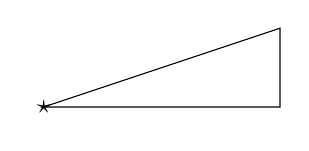
\begin{tikzpicture}
        % Draw triangle.
        \draw (0,0) -- (3,0) -- (3, 1) -- cycle;
        % Draw text.
        \node at (0,0) {$\star$};
    \end{tikzpicture}
}

\begin{figure}[h!]
    \centering
    \begin{minipage}{.5\linewidth}
        \centering
      	\subfloat[]{
            \label{:a}
            \pictureOne
      	}
    \end{minipage}%
    \begin{minipage}{.5\linewidth}
        \centering
      	\subfloat[]{
            \label{:b}
            \pictureTwo
      	}
    \end{minipage}
    \caption{}
    \label{}
\end{figure}
